\documentclass[letterpaper]{article}
% Used to do math and such (I think...)
\usepackage{amsmath}
\usepackage{amssymb}

% Used to color text (for todos)
\usepackage{xcolor}

% Used to embed pdfs from yEd and other sources
\usepackage{graphicx}

% Used to embed gnuplot output into document
\usepackage{epstopdf}

% Used to have a table span multiple pages.
\usepackage{longtable}

\usepackage{listings}

\usepackage{pdflscape}
\usepackage{geometry}

\usepackage{listingsutf8}
\usepackage{array}
\usepackage{multicol}
\usepackage{multirow}

\usepackage{algorithm}
\usepackage{algpseudocode}

\usepackage{float}

\usepackage{xspace}

\usepackage{subfig}
\usepackage{wrapfig}



% Deal with backwards quotes because evidently Latex doesn't know better.
\usepackage [english]{babel}
\usepackage [autostyle, english = american]{csquotes}
\MakeOuterQuote{"}

\usepackage{mathrsfs}

\DeclareMathOperator{\trace}{Tr}
\DeclareMathOperator{\argmax}{argmax}

\newcommand{\Erdos}{Erd\H{o}s\xspace}
\newcommand{\Renyi}{R\'enyi\xspace}
\newcommand{\Prob}[1]{\mathbb{P}\left( #1 \right)}
\newcommand{\Expected}[1]{\mathbb{E}\left( #1 \right)}

\newcommand{\Derivative}[1]{ \frac{d}{d #1} }
\newcommand{\NDerivative}[2]{ \frac{d^{#2}}{d #1^{#2}}}
\newcommand{\PartialDer}[1]{ \frac{\partial}{\partial #1} }
\newcommand{\NPartialDer}[2]{ \frac{\partial^{#2}}{\partial #1^{#2}} }

\newcommand{\NetworksEq}[2]{Eq. (#1) p. #2 of \textit{Networks} }
\newcommand{\NetworksFig}[2]{Fig. (#1) p. #2 of \textit{Networks} }
\newcommand{\NetworksSec}[2]{\S #1 p. #2 of \textit{Networks}}

\newcommand{\Floor}[1]{\left \lfloor #1 \right \rfloor}

\newcommand{\TODO}[1]{\textcolor{red}{#1}}

\newgeometry{margin=1.125in}

\begin{document}

\title{CSCI-5622: When They Buzz}
\author{Alex Gendreau \and Garrett Lewellen \and Tyler Behm \and a.k.a. Team Skynet}
\date{May 7\textsuperscript{th}, 2015}

\maketitle

\section{Problem}

\paragraph{} Contestants in a quiz bowl may answer a question as it is being read by buzzing in. We wish to predict when this will happen so that an artificial agent will buzz in just before other contestants. We treat this as two separate problems 1) at what point in the question will the user buzz in, and 2) will the user answer correctly. Correctly answered positions will be reported with a positive sign, and incorrectly negatively. We measure (1) by root mean square error (RMSE) and (2) by sign accuracy (ACC).

\section{Original Approach}

\paragraph{} We originally proposed a user-dependent probabilistic model based on independence assumptions to report the position with the highest probability given question features. Using logistic regression we found the approach slow and inaccurate (RMSE 106). We pivoted in favor of two simpler parallel lines of work: the Expected Value approach and Right-Wrong approach.

\section{Expected Value Approach}

\begin{figure}[H]
	\begin{center}
		\resizebox{0.8\linewidth}{!}{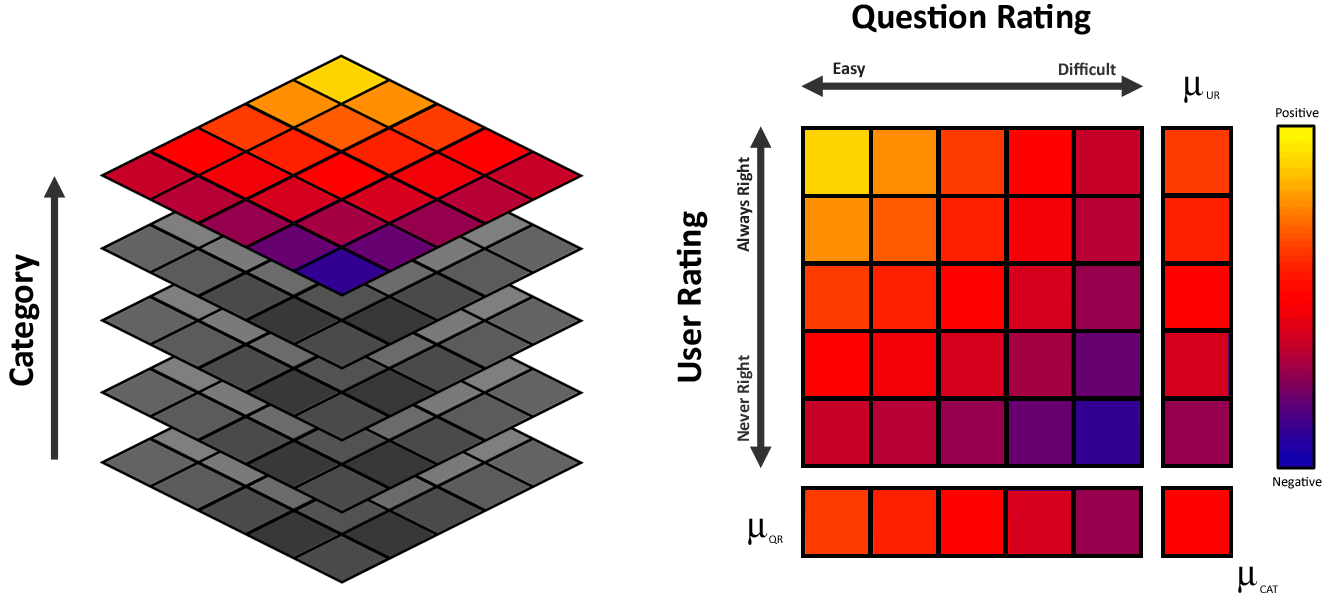
\includegraphics{expectedModel.png}}
	\end{center}
	\caption{Visual representation of the approach. If user rating or question rating are unknown, then expected positions $\mu_{QR}$ and $\mu_{UR}$ are used, or $\mu_{CAT}$ if neither is known.}
	\label{fig:expectedValue}
\end{figure}

\paragraph{} Garrett's simplest approach reported the expected position based on category, user rating, and question rating as depicted in Fig. (\ref{fig:expectedValue}). Users' abilities are measured by the portion of questions they answer correctly denoted by an integer value in $[-7, 7]$. Questions' difficulties are similar, but measured by portion of users who answer them correctly denoted by an integer in $[-2, 2]$. Garrett believed these features ultimately influenced the resulting sign and position. Result: RMSE of 87.48 and ACC of 72.50\%.

\begin{figure}[H]
	\begin{center}
		\resizebox{0.7\linewidth}{!}{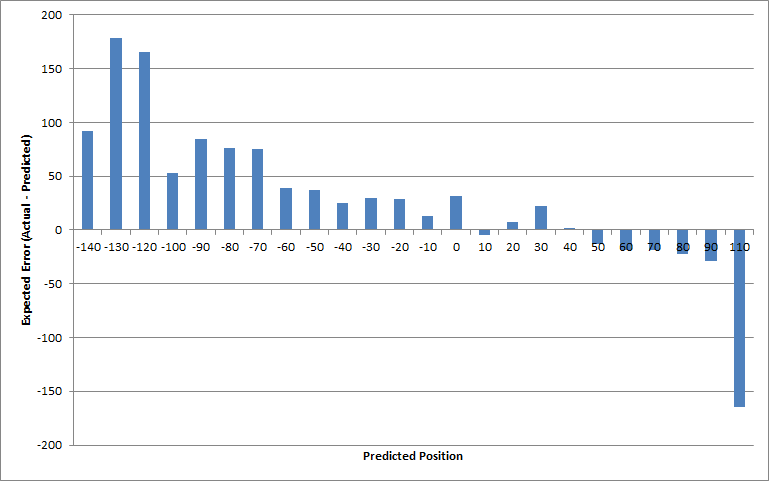
\includegraphics{expectedModelErrorAnalysis.png}}
	\end{center}
	\caption{Expected error as a function of predicted value.}
	\label{fig:expectedValue:errorAnalysis}
\end{figure}

\paragraph{} To improve RMSE, Garrett looked at the relationship between expected error and predicted position. With the intent to zero expected error, he applied these errors as position corrections to produce RMSE of 84.39 and ACC of 73.02\%. Repeating the process three more times yielded RMSE of 83.73 and ACC of 72.65\%. Next, he looked at the most frequently reported position, user rating, and question rating to apply further corrections based on category to obtain RMSE of 83.25 and sign accuracy of 73.5\%.

\begin{figure}[H]
	\begin{center}
		\resizebox{\linewidth}{!}{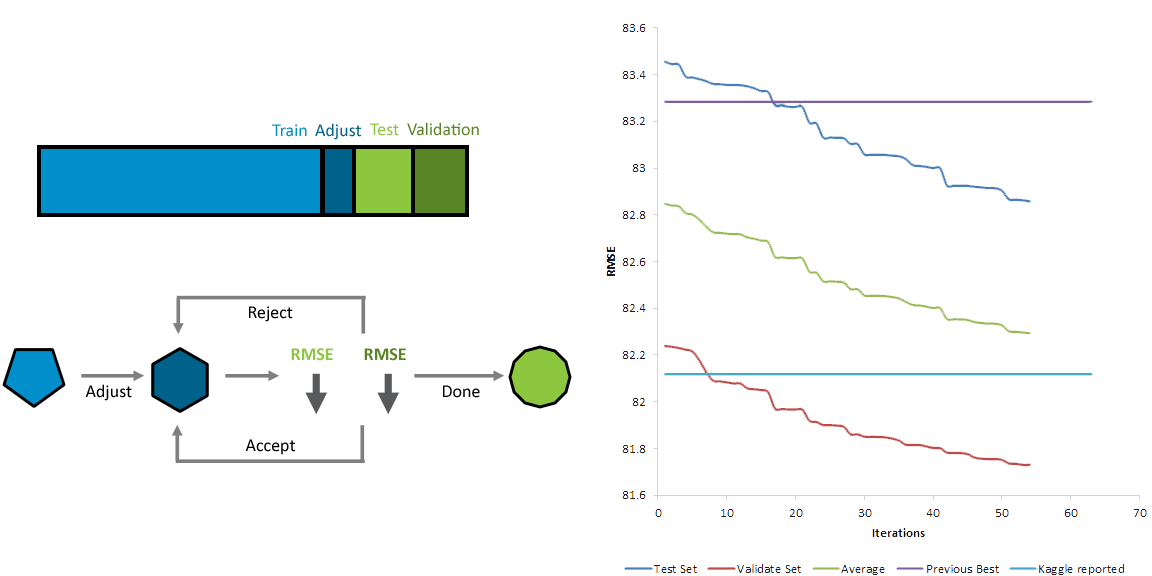
\includegraphics{expectedModelRefinement.png}}
	\end{center}
	\caption{(Left) Visual representation of refinement algorithm. (Right) RMSE as a function of algorithm iteration.}
	\label{fig:expectedValue:refinement}
\end{figure}

Finally, he automated this adjustment process as depicted in Fig. (\ref{fig:expectedValue:refinement}) by splitting the training set into four sets: two to initially fit and adjust the model, and two to verify adjustments reduced RMSE on two separate sets to mimic the Kaggle setup. From the initial fit, examples from the adjustment set are used to make corrections to the model. If RMSE does not improve for both test sets, an adjustment is rejected, otherwise it is accepted, and the process continues until the adjustment set is exhausted. Result: RMSE of 82.11832 as our best Kaggle score until May 2\textsuperscript{nd}.

\section{Right-Wrong Approach}

\paragraph{} Tyler was the first to realize that incorrectly predicting whether an answer was right or wrong has a higher penalty to the RMSE than the absolute value of the position. This is because of the bimodal distribution of answer positions. See Fig. \ref{fig:categoryPositions}.


\begin{figure}[H]
	\begin{center}
		\resizebox{0.7\linewidth}{!}{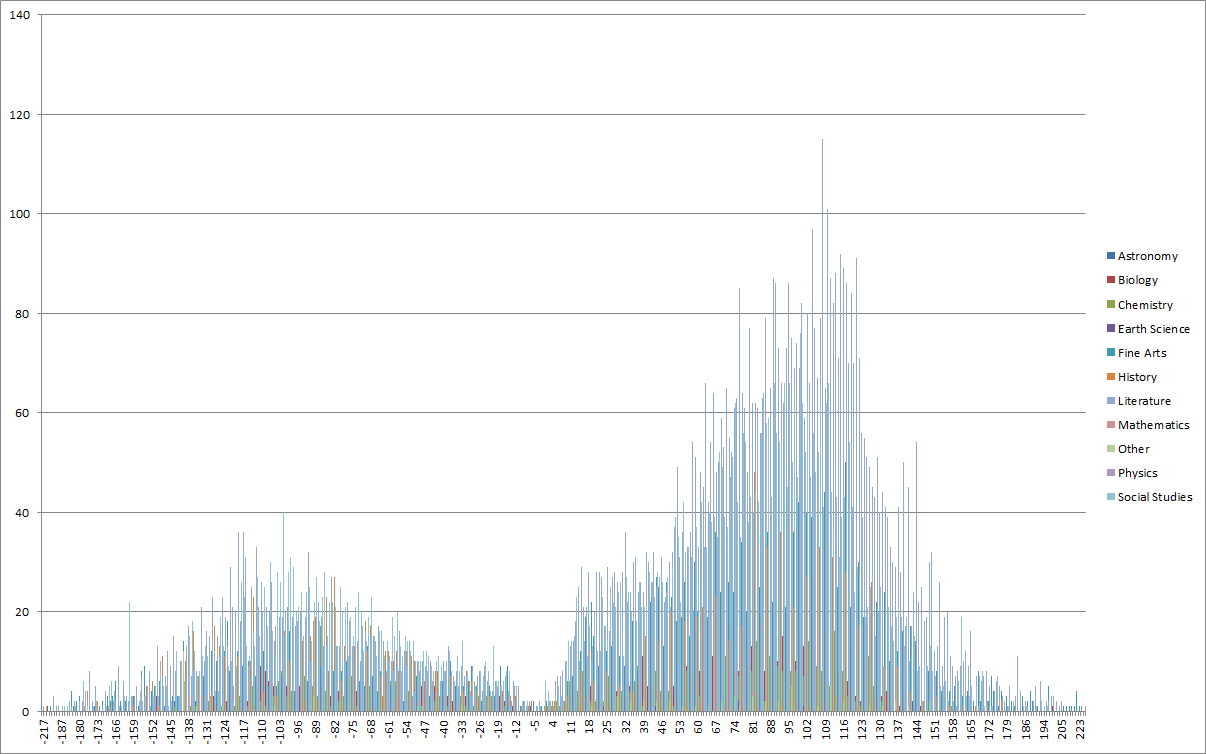
\includegraphics{categoryPositions.png}}
	\end{center}
	\caption{Histogram of frequency of answers binned by answer positions and separated by category.}
	\label{fig:categoryPositions}
\end{figure}

Thus, right-wrong predictions warrant their own logistic regression classifier. The following plots motivate the effectiveness of the features. User id was not an effective feature. The histogram shows that most user ids answered few questions. See Fig. \ref{fig:userHisto}. Category was an effective feature. The bar graph shows that the literature category has an average position of twice that of mathematics. See Fig. \ref{fig:categoryAverages}. This could be because literature questions were answered later than math questions, because literature questions were answered correctly more often than math questions, or because of some combination of the two factors. 

The initial implementation of the right-wrong approach modified the original guess file. The original guess file predicted the mean of the training set (39.298062750052644) for all test values. By negating the sign for each prediction in this file, this first implementation by Tyler improved the team's public Kaggle score to 84.27541 which was best so far for the team by April 14\textsuperscript{th}.

Later implementations of the right-wrong approach took the position prediction from the expected value approach as a feature. We tried using it vice-versa (right-wrong as feature into expected) but this was unsuccessful.

The right-wrong approach contributed to the improvements of future models. We used the right-wrong and expected approach to make a combined approach that earned a kaggle score of 86.94926 on April 30\textsuperscript{th}. This indicated that further efforts and innovations were needed to integrate these two models. This innovation was the continuum of correctness approach of which the right-wrong approach was the predecessor. By separating the problem to be solved into sign and position, we were able to give the sign its own model. This allowed us to feed position into it as an additional predictor and to tailor the regression learning specifically to the prediction of correctness. Thus, this approach improved the RMSE of our final model.



\begin{figure}[H]
	\begin{center}
		\resizebox{0.7\linewidth}{!}{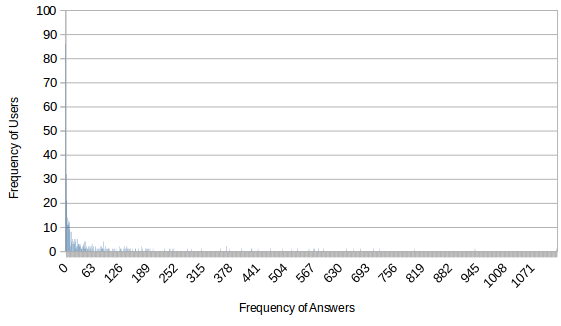
\includegraphics{histogram.png}}
	\end{center}
	\caption{Histogram of frequency of users binned by number of questions they answered.}
	\label{fig:userHisto}
\end{figure}

\begin{figure}[H]
	\begin{center}
		\resizebox{0.7\linewidth}{!}{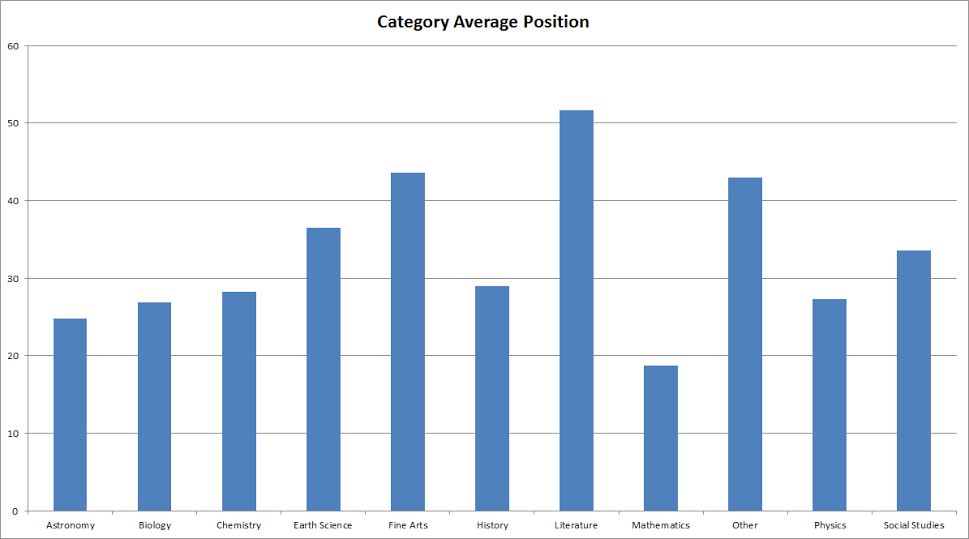
\includegraphics{categoryAverages.png}}
	\end{center}
	\caption{Bar graph of average answer position for each category.}
	\label{fig:categoryAverages}
\end{figure}

\section{Final Approach}

\paragraph{} Because incorrectly predicting whether an answer was right or wrong has such a high penalty, we chose to explore a continuum of correctness predictions. This would allow us to hedge our bets based on how confident was the right-wrong classifier.

\begin{minipage}{3in}
\begin{verbatim}
def hedge_bets(guess, conf, mean = 39.298062750052644):
    ## diff is between 0 (no confidence) and 1 (high confidence)
    ## it is the difference in probabilities for predicting yes and no, respectively
    ## output is confidence-weight position guess
    ## the less confident the guess, the more it is dragged towards the mean
    diff = abs(conf[0] - conf[1]) 
    return guess*diff + mean*(1 - diff)
\end{verbatim}
\end{minipage}

\paragraph{}

Tyler's first approach of this is shown in the code snippet above. It is a confidence-based linear interpolation towards the mean of the training set. If the right-wrong classifier was $100\%$ certain of its prediction, then the exact position classifier's prediction is returned. If the right-wrong classifier was evenly split between the right and wrong prediction, then the mean is returned. This reduces our risk of increasing the RMSE for low confidence right-wrong predictions.

Continuing with the approach above, Alex approached the problem of predicting the position and correctness of the answer as two separate sub problems.  First she learns the positions and then using the learned position as an additional feature, she learns the correctness.  

From the previous models two particular issues came to our attention
\begin{enumerate}
\item Overfitting of the training data
\item Harsh penalty for predicting the wrong correctness value as mentioned above
\end{enumerate}

To counteract the first issue, Alex decided to remove the user id and question id as features and return to a simpler model that used only information contained in the question to predict the position to prevent overfitting of the training data.  For more information as this model, see Section~\ref{sec:pp}.  To counteract the second issue, she decided that while correctness is a categorical variable, the model does not have to treat it as one especially since the current model is not especially good a predicting the correctness.  Building on the "hedging our bets" approach as described above, she chose to predict the confidence in the correctness on a sliding scale from $[-1,1]$.  For more information on this approach, see Section ~\ref{sec:pc}.

\subsection{Predicting Position}
\label{sec:pp}
\paragraph{}To prevent overfitting on the training set, Alex decided to use a small set of features based on the question and use regression to predict the absolute position of the answer.  The following features are used to predict the absolute position...
\begin{itemize}
\item Question Length (number of words)
\item Category
\item Correct Answer
\item Number of Hints
\end{itemize}
The first three features are given in the question text, but the hints are a feature that we defined ourselves.  From examining the data, we noticed that each question is phrased similarly (a set of facts (or hints) describing the answer that are separated by punctuation or conjunctions (and, or).  An answer is usually given following a hint.  We currently have a rudimentary way of predicting the total number of hints in the question.  We count the number of words each sentence that are proceeded by punctuation or conjunctions.  The method of predicting hints proved useful in predicting the position (one of the top five features), see Figure 8.  This method could potentially be refined into a better feature.

\lstset{
  basicstyle=\itshape
  }

To convert the categorical features of category and correct answer into numerical features that can be used by \lstinline{sk-learn}, Alex used the DictVectorizer to generate a feature matrix.  The target set is the absolute position of the answer.  Alex tried a variety of regression algorithms (linear, lasso, and ridge) varying the $\alpha$ parameter by factors of $10$ for both lasso and ridge regression.  She found that the using lasso regression with $\alpha=0.1$ to produce the best RMSE in terms of absolute position using a randomly selected cross validation set ($40\%$ of training data removed to be used as test data).  We believe that Lasso Regression worked the best since using the correct question answers leads to a large yet sparse feature set.

\subsection{Predicting Correctness Continuum}
\label{sec:pc}
\paragraph{} After predicting the absolute answer position, we need to determine the correctness of the answer.  Since incorrect predictions contribute significantly to the RMSE, Alex decided to predict the confidence in as a number between $[-1,1]$ and the multiply the predicted absolute position by this confidence to determine the final position/correctness prediction.  Ideally if the model is 100\% certain in the correctness then the position will only change in sign based on correctness.  However as is the case with most questions, the model is not certain in the correctness by multiplying the position by a number less than one, the position moves closer to 0 and thus decreases the penalty for an incorrect correctness prediction.  For this model, the same features were used as those to predict the absolute position in Section ~\ref{sec:pp} with the addition of the absolute position as a feature.  The targets are $\pm 1$.

Since the goal was to predict continuous output that represents the confidence of the correctness prediction, Alex again chose to use a regression model.  Similar to predicting the absolute position, she experimented with linear, lasso, and ridge regression while varying the $\alpha$ parameters by factors of $10$ for lasso and ridge regression.  She found that ridge regression with $\alpha=5$ minimized the RMSE on the cross validation set as described in Section ~\ref{sec:pp}.  Ridge regression prevents any feature from contributing a large factor to the final results.  While this proved the best model on the training data, it suffers from overfitting issues that are discussing in Section ~\ref{sec:micro}.

The two part model described above produced the best Kaggle score and was the final submission for our team.  For an illustration of correctness continuum, see Figure \ref{fig:corr_cont}.  

\begin{figure}[H]
	\begin{center}
		\resizebox{0.7\linewidth}{!}{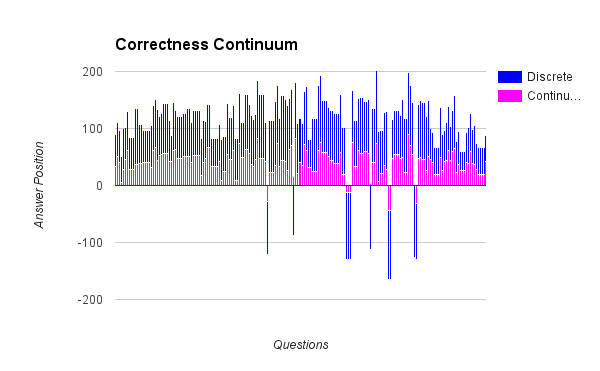
\includegraphics{correctness_cont.png}}
	\end{center}
	\caption{The difference in position based on using logistic regression for modeling the correctness (Discrete) and ridge regression (continuous).}
	\label{fig:corr_cont}
\end{figure}

\section{Error analysis}
\paragraph{} Error analysis occurs at two different levels.  The macro level, Section ~\ref{sec:macro}, examines error on the entire data set or large subcategories to determine how well the model predicts the data on average.  The micro level, Section ~\ref{sec:micro}, examines why the model is especially bad at predicting certain examples.  Both of these error analyses can aid in determining the most influential features and provide guidance in developing new features.  

Figure 8 represents the largest contributing features to the position model.  We see three categories as the largest features.  This is not unexpected since these three categories are the largest in the training set.  

\begin{figure}
\centering
\begin{minipage}[t]{.4\textwidth}
%\begin{table}[tb]
\centering
\vspace{0pt}
%\begin{table}[tb]
%\centering
\begin{tabular}{|l |}
\hline
Position Feature Weights \\ \hline
Literature (2.48) \\
History (1.17) \\
Fine Arts (-1.03) \\
Question Size (0.79) \\
Total Hints (-0.17) \\ \hline
\end{tabular}
\caption{The five features whose coefficient is larger than $0.001$ for the model which predicts the absolute answer position}
\label{table:pos_feat}
%\end{table}
\end{minipage}\hfill
\begin{minipage}[t]{.4\textwidth}
\centering
\vspace{0pt}

%\begin{table}[tb]
%\centering
\begin{tabular}{cc|c|c|}
\cline{3-4}
& & \multicolumn{2}{ c| }{Predicted} \\ \cline{3-4}
& & -1 & +1 \\ \cline{1-4}
\multicolumn{1}{ |c  }{\multirow{2}{*}{Actual} } &
\multicolumn{1}{ |c| }{-1} & 4.8 & 22.2      \\ \cline{2-4}
\multicolumn{1}{ |c  }{}                        &
\multicolumn{1}{ |c| }{+1} & 3.5 & 69.5     \\ \cline{1-4}


\end{tabular}







\caption{The predictions from the correctness continuum.}
\label{table:pos_feat}
%\end{table}
\end{minipage}
\end{figure}

\subsection{Macro Level}
\label{sec:macro}

\paragraph{} We examine errors in both position and correctness.  In Figure \ref{fig:abs_off} which is average difference between absolute predicted position and absolute actual position by category.  Unfortunately this graph is not very telling since all the categories are similar in terms of difference.  From this we can see that category while good for predicting the position is not causing significant error in one category.

We now turn to correctness, which was the main focus of a lot of our efforts since it was such a large factor of the RMSE.  In Figure \ref{fig:corr_off}, we see the percent of questions that are incorrectly predicted correct/incorrect by category.  Here we do see some trends such as Earth Science and Mathematics are more likely to have incorrect correctness predictions whereas Literature and Other are more likely to have correct correctness answers.  Since we in general are predicting more significantly more false positives than false negatives, see Figure 9.  This could lead to us adding more weight to the Mathematics category that favors incorrect answers.  


%\begin{figure}[H]
%	\begin{center}
%		\resizebox{0.7\linewidth}{!}{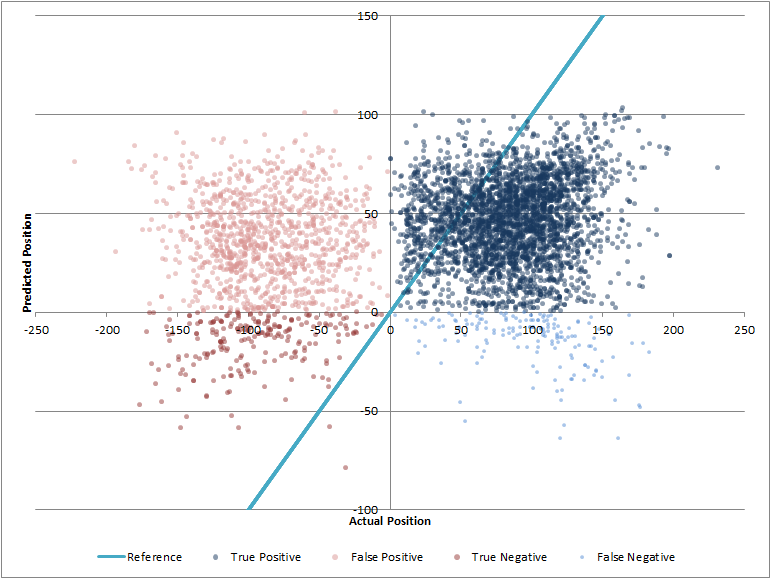
\includegraphics{confidence.png}}
%	\end{center}
%	\caption{Confidence in Correctness}
%	\label{fig:mircoH}
%\end{figure}

\begin{figure}[H]
	\begin{center}
		\resizebox{0.7\linewidth}{!}{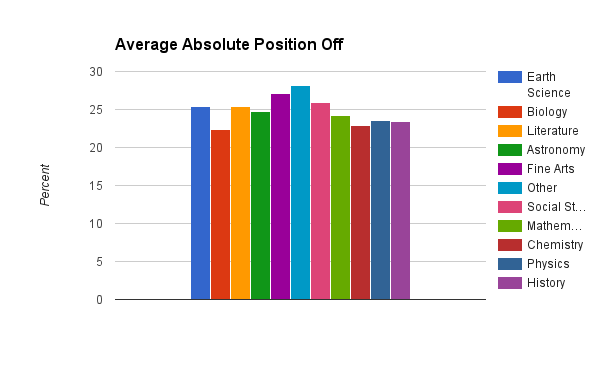
\includegraphics{absolute_pos_off.png}}
	\end{center}
	\caption{Position off by Category}
	\label{fig:abs_off}
\end{figure}

\begin{figure}[H]
	\begin{center}
		\resizebox{0.7\linewidth}{!}{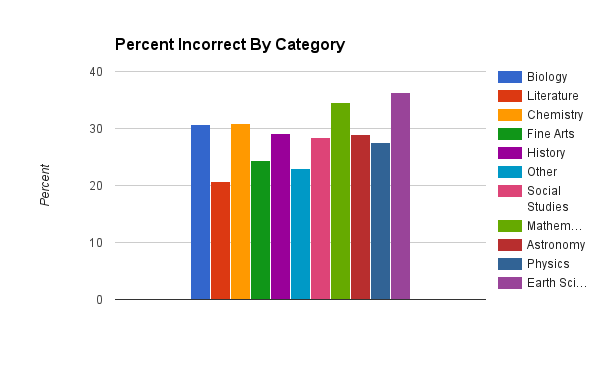
\includegraphics{wrong_correctness.png}}
	\end{center}
	\caption{Correctness of by category}
	\label{fig:corr_off}
\end{figure}

\subsection{Micro Level}
\label{sec:micro}
\paragraph{} For the micro level analysis we examine two specific questions that contribute large values to our RMSE.  First we examine an example where the absolute position from stage 1 of the position/correctness prediction, see Figure 12 and Table 1.  Here the issue is that the question was answered incorrectly (on average smaller position than correct answer) and the question was longer than average for fine arts questions.  The increased length plus the smaller incorrect answer lead to the position predicted to be too large.  One thing to take away from this is that potentially predicting absolute position is not the best way to go since correctness can effect the relative position. 

The false positives in terms of correctness are the largest factor in our RMSE.  This category is hard to predict since there are more correct questions than incorrect questions.  

\begin{figure}[H]
\centering
\begin{minipage}[t]{.4\textwidth}
%\begin{table}[tb]
\centering
\vspace{0pt}

\begin{tabular}{|l|l |}
\hline
Category & Fine Arts \\ \hline
Length &  223 \\
Hints & 12 \\
Predicted Position & 171.46 \\
Actual Position & 46 (Incorrect) \\ \hline

\end{tabular}
\captionof{table}{The information for question 115661.}
\label{table:ex_art}
%\end{table}
\end{minipage}\hfill
\begin{minipage}[t]{.4\textwidth}
\centering
\vspace{0pt}
%\begin{figure}[H]
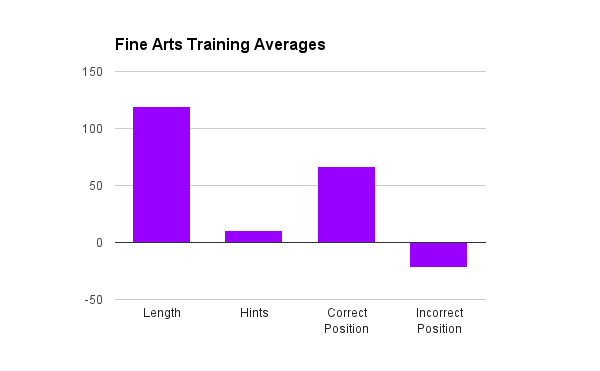
\includegraphics[width=\textwidth]{finearts.png}
\caption{Breakdown of the training fine arts category}
\label{fig:mircoFA}
%\end{figure}
\end{minipage}

\end{figure}

The next example Alex investigated is an example that contributes greatly to the overall RMSE in Table 2 and Figure 13.  This example is an example of an overfitting issue of our correctness model.  Since we include the correct answer as a feature, a question with the answer, Louis XI, appeared incorrectly in the training set whereas the user answered this question correctly.  However since the training data has this answer as incorrect with a relatively large weight ($-0.19$), the model is very unsure whether the answer is correct or not pushing the position near $0$. 

\begin{figure}
\centering
\begin{minipage}[t]{.4\textwidth}
%\begin{table}[tb]
\centering
\vspace{0pt}

\begin{tabular}{|l|l |}
\hline
Category & History \\ \hline
Length &  179 \\
Hints & 19 \\
Predicted Position & 12.82 \\
Actual Position & 179\\ 
Predicted Absolute & 137.49 \\ 
Correctness Coefficient & 0.093 \\
Answer & Louis XI \\ \hline

\end{tabular}
\captionof{table}{The information for question 122925}
%\label{table:ex_art}
%\end{table}
\end{minipage}\hfill
\begin{minipage}[t]{.4\textwidth}
\centering
\vspace{0pt}
%\begin{figure}[H]
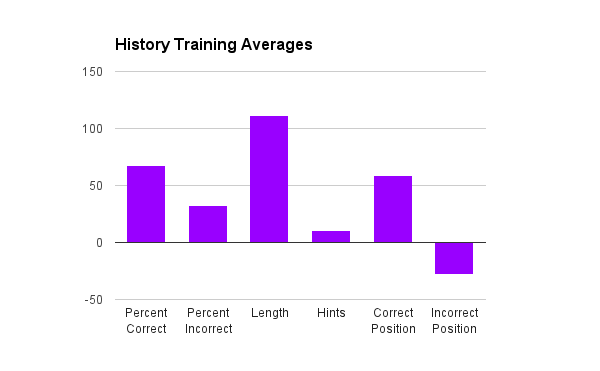
\includegraphics[width=\textwidth]{history.png}
\caption{Breakdown of the training history category}
\label{fig:mircoH}
%\end{figure}
\end{minipage}
\end{figure}




\section{Conclusions}

\paragraph{} On the public leaderboard, our team placed 4th among 10 teams with a score of 81.55. On the private leaderboard, our team placed 5th with a score of 82.98. Our drop in rank from public to private indicates some degree of overtraining on the public test data. 

To improve our model in the future, we need to determine features that are better able to predict correctness.  One potential way of doing this is making use of the specific user and question information.  While using this information in the general model let to overfitting of the training set, we should employ this information to either generate separate models for known users and questions individually or through clustering users who answer similar questions.  We could also include this information as a post-processing step after applying the general model.

\end{document}
